%%%%%%%%%%%%%%%%%%%%%%%%%%%%%%%%%%%%%%%%%%%%%%%%%%%%%%%%%%%%%%%%%%%%%%%%%%%%%%%%
%2345678901234567890123456789012345678901234567890123456789012345678901234567890
%        1         2         3         4         5         6         7         8

\documentclass[letterpaper, 10 pt, conference]{ieeeconf}  % Comment this line out if you need a4paper

%\documentclass[a4paper, 10pt, conference]{ieeeconf}      % Use this line for a4 paper

\IEEEoverridecommandlockouts                              % This command is only needed if 
                                                          % you want to use the \thanks command

\overrideIEEEmargins                                      % Needed to meet printer requirements.

% See the \addtolength command later in the file to balance the column lengths
% on the last page of the document

% The following packages can be found on http:\\www.ctan.org
\usepackage{graphics} % for pdf, bitmapped graphics files
\usepackage[pdftex]{graphicx}
%\usepackage{graphicx}
\usepackage{epsfig} % for postscript graphics files
\usepackage{mathptmx} % assumes new font selection scheme installed
\usepackage{epstopdf}
\usepackage{times} % assumes new font selection scheme installed
\usepackage{amsmath} % assumes amsmath package installed
\usepackage{amssymb}  % assumes amsmath package installed
\usepackage{cite}



\begin{document}

\section{GARDEN DESIGN}

\subsection{Overview}

In this section, we introduce the overall hardware system of the origami-inspired robotic flower garden. The garden bed has six rows and three columns for 16 tiles, which are full of robotic flowers (Fig. 1(a)). Each tile has 8-9 holes for connectors (Fig. 1(b)).

One set of robotic flower has many mechanical and electrical components (Fig 2), which are as follows:

\begin{itemize}
	\item Origami flower: flowers are made of thin color papers or thin acrylic plates. The designed flowers are manually cut and folded.
	\item Pouch motors: pouch motors are soft pneumatic actuators used to actuate the blooming motion of petals. Their shape, dimension and patterns are programmed in a desktop computer, and manufactured by using the heat sealing method\cite{NiiyamaICRA2014}.
	\item Tubes and wires: Tubes and wires provide electric signals and air pressure to the flowers. They are made by coated by green-colored liquid rubber and cured in a room temperature for a day. The rubber coating increases the stiffness of the stem, and the flower and stem can maintain its pose. 
	\item Connector: the connector has three functions. First, it makes the rubber-coated stem fixed on the plate. Second, it connects the air pressure and electric signals from the system below the tile to the air pouch and LEDs in the flower. Finally, a broken flower is pulled out and exchanged to a new one easily (see the right flower in Fig. 2). Connectors are made by using a 3-D printer or rubber molds.  
	\item Acrylic plate: the plate has 8-9 holes, which are for connectors. The position of holes can be programmed in a CAD tool, and they are rapidly manufactured by using a laser cutter.
	\item Pneumatic and electrical system: Each tile has one pneumatic and electrical setup to actuate the pneumatic pouch and LEDs inside the flower. Details about this setup is introduced in the section II.C.  
\end{itemize}

\begin{figure}[thpb]
	\centering
	\includegraphics[scale=.45]{figures/tabletile.jpg}
	\caption{(a)The robotic garden bed is consisted of 16 identical modular tiles. (b) the top view of a modular tile}
	\label{tabletile}
\end{figure}

\begin{figure}[thpb]
	\centering
	\includegraphics[scale=.4]{figures/connector.jpg}
	\caption{A schematic figure (side-view) of a pouch-actuated robotic flower. Each robotic flower has one connector, wires and a tube, printable and inflatable pouch, and LEDs (optional). The pneumatic and electrical system below the acrylic tile provides an air pressure and electric signals to the pouch and LEDs in the flower. It is possible to change the type and position of the robotic flowers from by pulling them. }
	\label{connector}
\end{figure}   

The above components are mass-producible using a laser cutter, a 3-D printer, a computer-controlled heal sealing machine, and molds.  Thus, we made 000 origami flowers, pouches and connectors, 16 tiles and pneumatic control systems [put the number]. Table 1 shows the specifications of the robotic garden. 

\subsection{Pouch Actuated Flowers}

The robotic flowers exhibited in the garden are all actuated by pouch motors. We made 8 types of flowers, of which 7 were folded with origami paper and 1 was made with acrylic plate and decorated with LEDs. They are: Tulip, Lotus, Lily, Spiral Flower, Bird of Paradise, Fireworks Flower, Clematis and the LED flower. In order to facilitate different foldings and to achieve different blossom effects, pouch motors are tailored to different designs and actuation mechanisms.

\begin{itemize}
	
	\item Tulip: Tulip has a pouch hided inside the side petals. When the pouch gets inflated, the originally folded pouch straightens and opens up the flower.
	\item Lotus: Inside Lotus, a smaller square pouch is stacked on top of a bigger square pouch. When they get inflated, they pushes up the stamen and pistils.
	\item Flower Lily: Flower lily has multiple pouches connected on a cross beneath the petals. Although the design looks like a linear mode pouch system as introduced by Niiyama et al. \cite{NiiyamaICRA2014}, it actually acts like discrete rotational mode single pouches, because the whole system is adhered to the petal not just the end of each pouch stems. When pouches are inflated, the individual pouches on the pouch stem ``bend'' the adhered paper petals to open.
	\item Spiral Flower: Unlike other robot followers on which pouch motors were adhered onto folded origami structures, we took a very different approach to make Spiral Flowers. For each Spiral Flower, we folded 12 simple petals and adhered them onto a spiral shape pouch. When the pouch inflates, the length of the spiral changes and presents a twisting effect on petals.
	\item Bird of Paradise: The actuation mechanism on the Bird of Paradises are similar to the one on Lotuses: Pouches are stacked. In this case, the bottom of the individual pouches are bonded together. When they are inflated, the pouches separates the petals to open.
	\item Fireworks Flower:  Like the Flower Lily, the pouch motors were hidden beneath the petals of the Fireworks Flower. The change in shape of the pouch during inflation pushes the flower to open.
	\item Clematis: Clematis used the same pouch motor design as the Lotus. The stamen and pistils are pushed outward with pouch inflation.
	\item LED Flower: Unlike the other flowers, the LED Flower is made with acrylic plates. There were one LED decorated on each petal. The blooming motion of the petals are actuated by rotational mode single unit pouch motors, which was discussed in details by Niiyama et al. \cite{NiiyamaICRA2014}. The wires connecting the LEDs were wrapped around the stem down onto a plug connector. 
	
\end{itemize}

\begin{figure}[thpb]
	\centering
	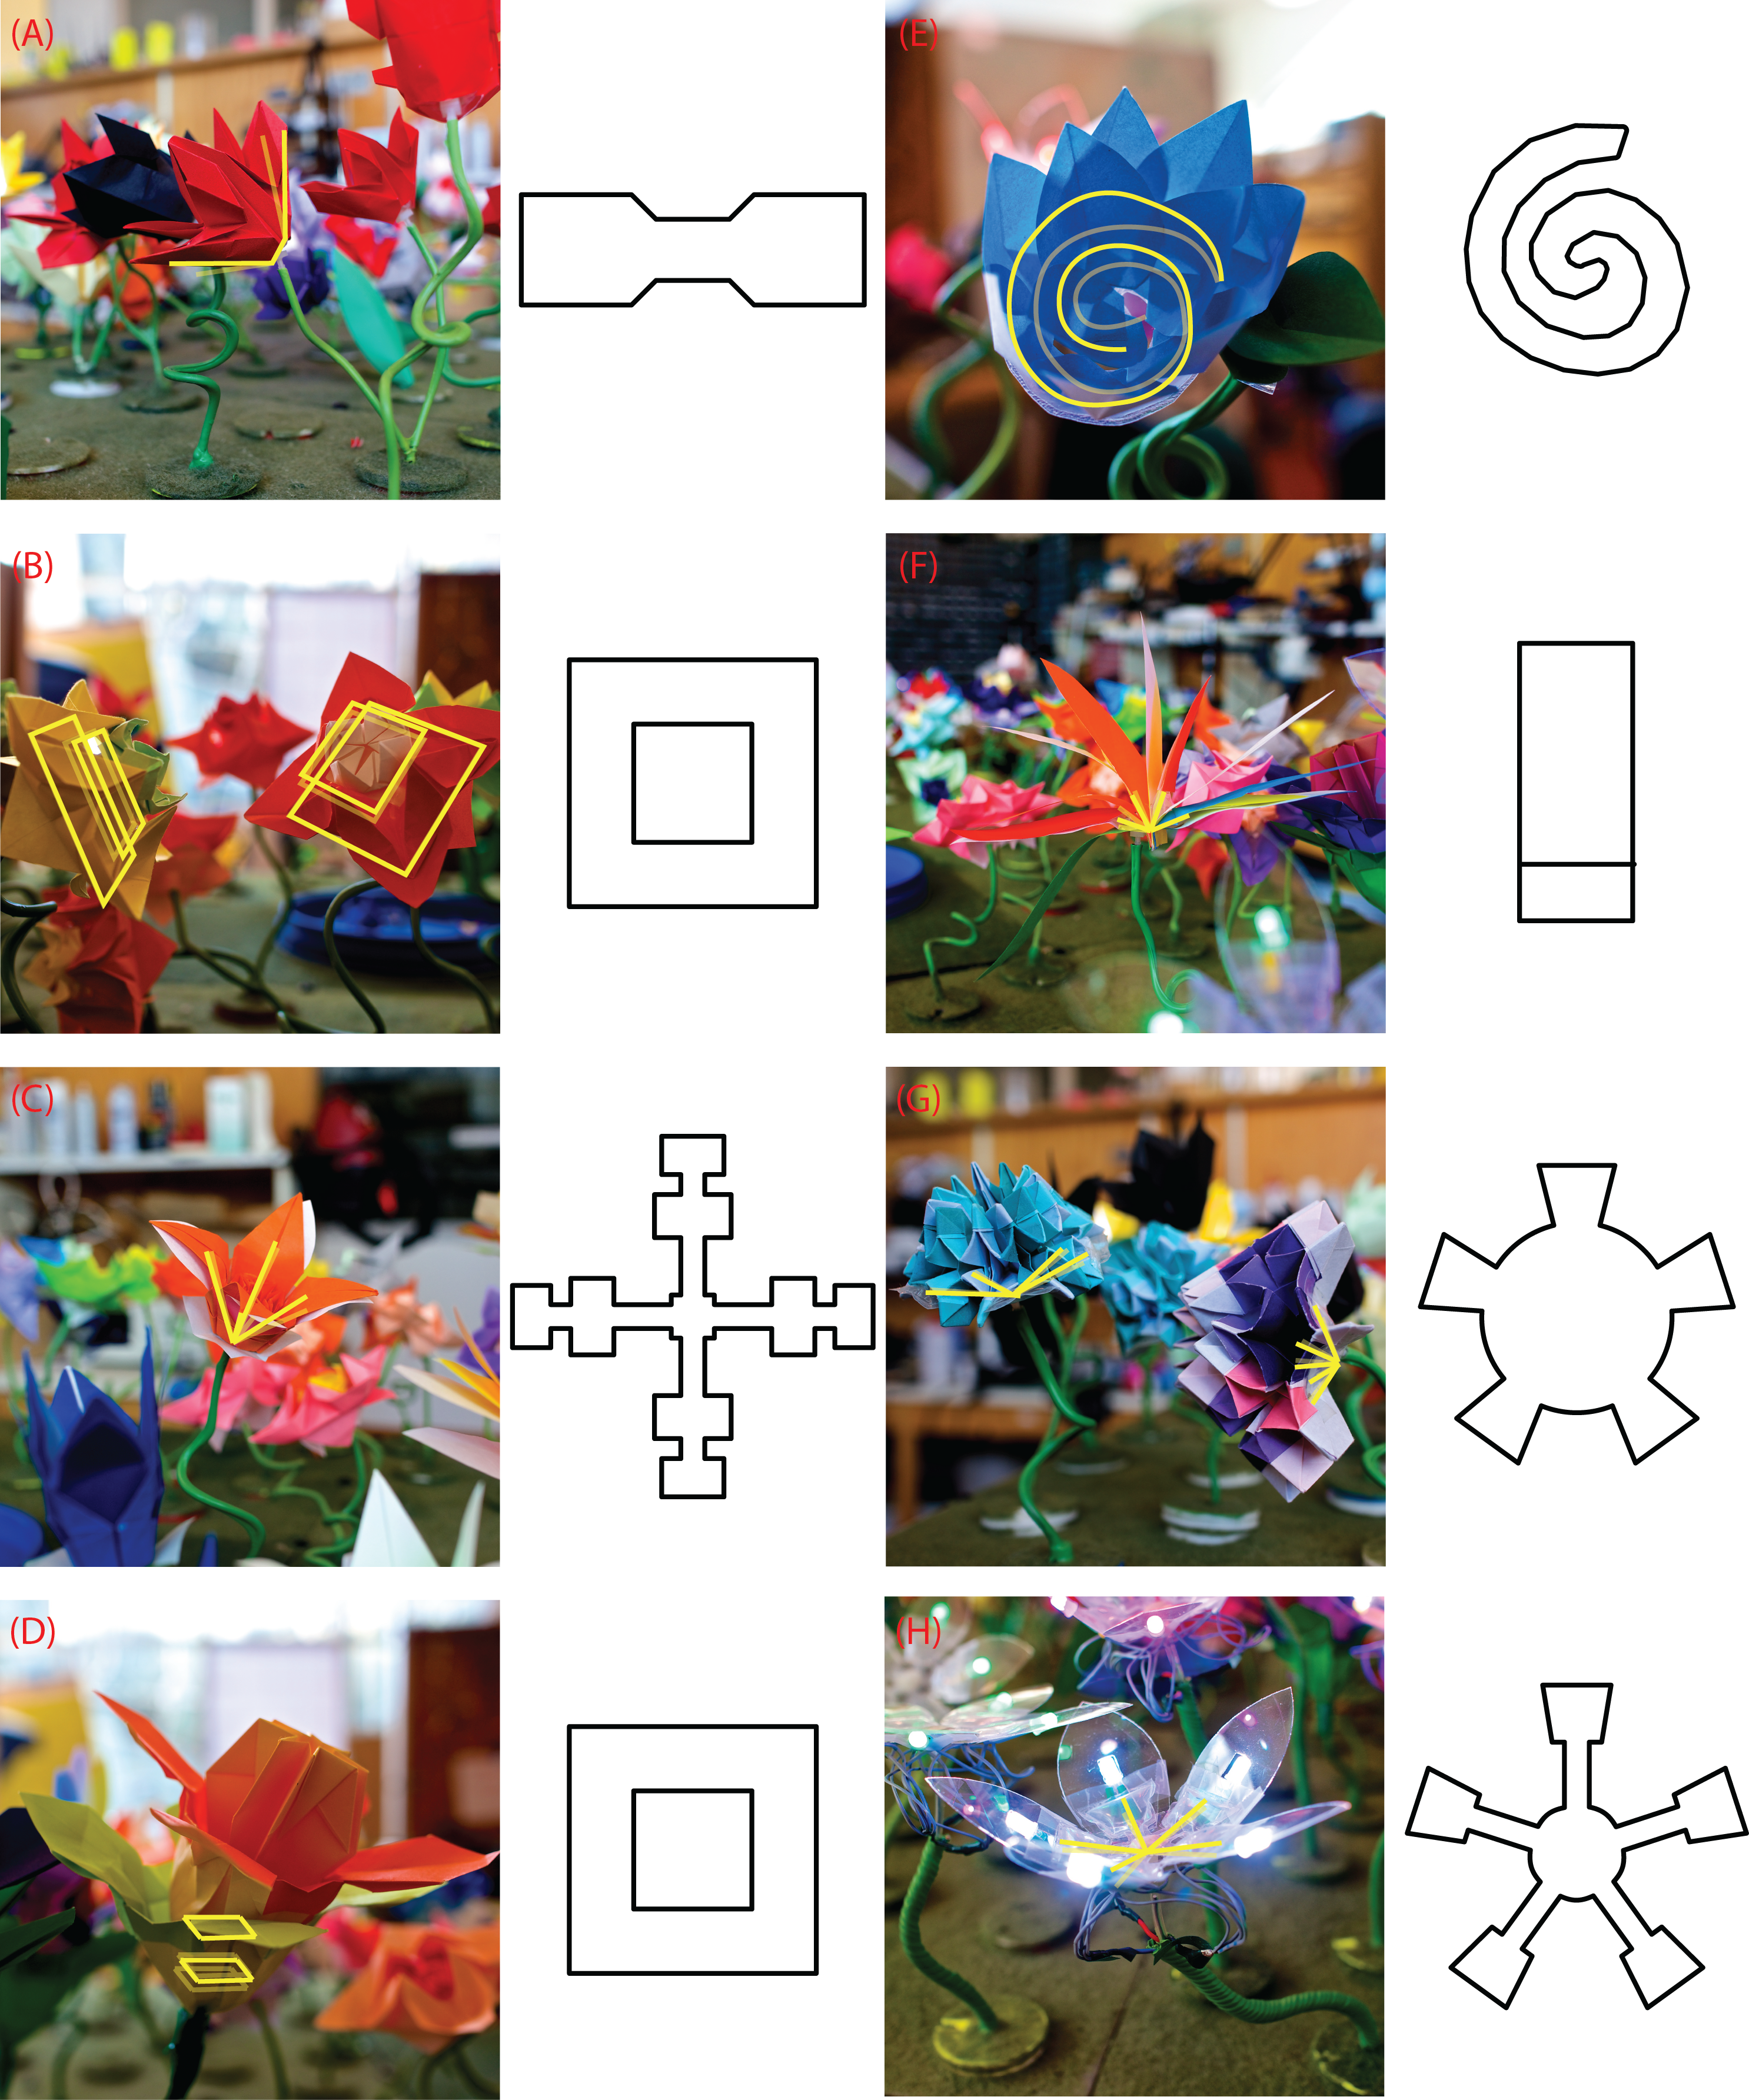
\includegraphics[scale=.22]{figures/flowers.png}
	\caption{pictures of flowers at pouch inflations and corresponding pouch motor design. The locations of the pouches are marked in yellow (A)Tulip (B) Lotus (C) Flower Lily (D) Clematis (E) Spiral Flower (F) Bird of Paradise (G) Fireworks Flower (H) the LED Flower }
	\label{flowers}
\end{figure}

\subsection{Computer-aided pouch motor designs and fabrication}

The versatile pouch motor making process used in this project allows us to iterate our designs quickly with variable scales. We designed pouch motors for each flower in a 2D CAD program. The design is then converted the drawing into Numerical Control (NC) codes. Finally, the NC codes are sent to a custom-made CNC machine to make pouch systems. This machine ``draws'' pouch patterns onto two layers of 4 mil thick polyethylene films at a time with a heated soldering iron \cite{NiiyamaIJRR2014}. %Both works submitted, not published

In the case of Lotus and Bird of Paradise, the pouches are stacked and interconnected. Thanks to the versatile fabrication process, these multilayer pouch motors can be made simply layer by layer. We added four alignment features on the CNC machine mounting board. We made the multilayer pouch by firstly making the ``air doors'' in between the neighbor pouches, and then thermally bonded the top pouch with fiberglass separating it from the bottom one.

\begin{figure}[thpb]
	\centering
	\includegraphics[scale=.25]{figures/doublepouch.png}
	\caption{An illustration of the fabrication method on a two-layer pouch motor}
	\label{doublepouch}
\end{figure}

% add a figure here - CNC machine photo?


%%%%%%%%%%%%%%%%%%%%%%%%%%%%%%%%%%%%%%%%%%%%%%%%%%%%%%%%%%%%%%%%%%%%%%%%%%%%%%%%


\addtolength{\textheight}{-12cm}   % This command serves to balance the column lengths
                                  % on the last page of the document manually. It shortens
                                  % the textheight of the last page by a suitable amount.
                                  % This command does not take effect until the next page
                                  % so it should come on the page before the last. Make
                                  % sure that you do not shorten the textheight too much.

%%%%%%%%%%%%%%%%%%%%%%%%%%%%%%%%%%%%%%%%%%%%%%%%%%%%%%%%%%%%%%%%%%%%%%%%%%%%%%%%

\bibliographystyle{IEEEtran}
\bibliography{bibfile}

\end{document}